% IEEE Paper Template for US-LETTER Page Size (V1)
% Sample Conference Paper using IEEE LaTeX style file for US-LETTER pagesize.
% Copyright (C) 2006 Causal Productions Pty Ltd.
% Permission is granted to distribute and revise this file provided that
% this header remains intact.
%
\documentclass{sig-alternate}
\usepackage{times,amsmath,epsfig,algorithm,algpseudocode,caption,subcaption}
\usepackage{color,url}

\newcommand{\secref}[1]{Section \ref{#1}}
\newcommand{\figref}[1]{Figure \ref{#1}}
\newcommand{\equref}[1]{Equation \ref{#1}}
\newcommand{\tabref}[1]{Table \ref{#1}}
%
\makeatletter
 \let\@copyrightspace\relax
\makeatother

\begin{document}
% --- Author Metadata here ---
\conferenceinfo{EDBT'13}{, Mar 18-22 2013, Genoa, Italy}
\CopyrightYear{2013} % Allows default copyright year (20XX) to be over-ridden - IF NEED BE.
\crdata{978-1-4503-1597-5/13/03}
% --- End of Author Metadata ---

\title{CISC: Clustered Image Search by Conceptualization}
%
\author{%
%% author names are typeset in 11pt, which is the default size in the author block
{Kaiqi Zhao{\small $~^{\#1}$}, Enxun Wei{\small $~^{\#1}$},
Qingyu Sui{\small $~^{\#1}$}, Kenny Q. Zhu{\small $~^{\#2}$}
\hspace*{-1mm}
\titlenote{Kenny Q. Zhu (corresponding author) is partially supported
by NSFC Grant 61100050 and 61033002.\vspace*{-5mm}}
}%
, Eric Lo{\small $~^{\dag3}$}
% add some space between author names and affils
\vspace{1.6mm}\\
\fontsize{10}{10}\selectfont\itshape
$~^{\#}$Shanghai Jiao Tong University\\
\fontsize{9}{9}\selectfont\ttfamily\upshape
$~^{1}$\{kaiqi\_zhao,nxun,sqybi\}@sjtu.edu.cn\\
\fontsize{9}{9}\selectfont\ttfamily\upshape
$~^{2}$kzhu@cs.sjtu.edu.cn\\
\fontsize{10}{10}\selectfont\itshape
$~^{\dag}$Hong Kong Polytechnic University\\
\fontsize{9}{9}\selectfont\ttfamily\upshape
$~^{3}$ericlo@comp.polyu.edu.hk\\
}


%%%

\maketitle

%\begin{abstract}
%  In the age of information explosion, search engines have been an
%  essential tool in people's daily life and query suggestion is one
%  of most useful feature for a standard search engine. However, because
%  most of search engines are keyword-based, many fantastic features would
%  fail when facing concept-based queries, so does query suggestion. In this
%  paper, we propose a framework so that search engines can give acceptable
%  suggestions when facing concept-based queries.
%\end{abstract}

\begin{abstract}
  A class of search queries which contain abstract concepts are studied in
this paper. These queries cannot be correctly interpreted by traditional keyword-based search engines.
  This paper presents a simple framework that detects and instantiates the
abstract concepts by their concrete entities or meanings to produce alternate
queries that yield better search results.
\footnote{Kenny Q. Zhu (corresponding author) is partially
supported by NSFC grants 61100050 and 61033002.}
\end{abstract}


\category{H.3.3}{INFORMATION STORAGE AND RETRIEVAL}{Information Search and Retrieval}
%\category{I.2.7}{ARTIFICIAL INTELLIGENCE}{Natural Language Processing}

\terms{Algorithms}

\keywords{Clustering, Image Search, Conceptualization}

\section{Introduction}

Protein$-$protein interactions (PPIs) are of central importance for the majority of biological functions, such as signal transduction, metabolic pathways, molecular dynamics, and protein networks\cite{Hoffmann.Krallinger.ea:2005}, for they serve as the most fundamental building blocks of the entire interacademic systems of any organisms. Collecting data on pairwise interaction relationships is essential for multiple purpose, including identification of modules with certain functionality\cite{Spirin.Mirny.03}, mapping diseases to dominated genes\cite{Ideker.Sharan.08}, and after all, understanding wholistic metabolic/genetic networks from a system biology perspective.

A lot of databases have been built to store protein and genetic interactions from major model organism species and are available in various standardized formats, such as MINT\cite{Zanzoni.Montecchi-Palazzi.ea:2002}, BIND\cite{Bader.ea:2003}, BIOGRID\cite{DBLP:journals/nar/StarkBRBBT06}, etc. Among those mainstream databases, the data largely rely on voluntary reports by scientists or researchers, besides, comprehensive curation efforts become indispensable for the sake of accuracy. However, the amount of biology-related literatures with respect to protein interactions grows explosively and thus make it either impossible or impractical to manually detect PPI information anymore.

Considering huge amount of PPI information with great wealth hidden in published papers, in recent years, numerous mining techniques have been proposed that aim to extract PPI information automatically from free text, especially machine learning, information retrieval, and natural language processing\cite{DBLP:journals/bib/WinnenburgWPDS08}.These approaches can be roughly categorized into three classes: co$-$occurrence, rule$-$based, and machine learning. 

Co$-$occurrence is the approach with most simplicity and naivete. Just as its name implies, this method intends to find out pairs of proteins that co-occur in the same context. The scope of "same context" ranges from phrase, sentence, paragraph to whole abstract, even document. The underlying assumption is that whenever two proteins are mentioned together by authors, chances are high that there is some kind of relationship between them. However, however, in-context closeness even semantic relation does not necessarily represent actual biological interaction. As a consequence, a large fraction of candidate pairs are mismatched inevitably, causing a high recall but low precision.

The second approach is rule-based extraction, in other words, pattern matching. There are many types of rules, most of them concern natural language processing (NLP). One way is to specify hand-crafted regular expressions before hand, which mostly lean on language usage preference. Besides, by using full or partial (shallow) parsing strategies, more information would be acquired, such as part-of-speech taggers, local dependencies between syntactic components, context-free grammar\cite{DBLP:journals/bioinformatics/TemkinG03}, and full sentence structure. Compared to co$-$occurrence, rule-based approach enjoy better precision but much lower recall. In addition, since the rules are usually derived from training data, that is to say, the improper choice of training data would be significantly lethal, therefore quality of extraction is invariably instable and may not applicable to other data.

The third and most commonly used approach use machine learning techniques, in this case, the task to extract protein$-$protein interactions turns out to be a binary classification problem. Each protein pairs are represented along with a set of features, which is associated with their context, then a well$-$defined classifier gives the answer whether the candidate protein pairs is classified to be qualified PPI. (TO BE FURTHER FILLED!!!)

In this paper, we introduce a general bootstrapping framework for Protein$-$protein interaction extraction from natural text.Our method differs from most of the previous works in three aspects:

(1)The extraction process is driven by only tiny fraction of training data, which are regarded as seed data. In each round, it would derive reliable patterns automatically from seed data, then extract more positive PPI pairs consequently, what's more, the seed data would be augmented by the newly extracted results with high confidence.

(2)multiple graph kernel. 

(3)various evaluation.




\section{Technical Specification}
\label{sec:tech}

\begin{figure}[h]
\begin{center}
\epsfig{file=archi.eps,width=0.85\columnwidth}
\caption{PredicTV System Architecture}
\shrink
\label{fig:archi}
\end{center}
\end{figure}

Figure \ref{fig:archi} illustrates the system architecture.
The core recommendation engine consists of two modules:
the offline web information extraction module and the online
recommendation module. The first module collects in advance weekly TV schedule,
identifies program titles and show times, and then extracts relevant
information about programs from web. 
The second module maintains user viewing model
dynamically and by comparing the similarity between the 
current user model and programs, 
recommends the most relevant programs to the user in real time.
We next present these two modules in greater details.

%Communication module receives users' channel switching requests,
%transfers them to Recommendation module, and outputs
%recommendations to the user. Database module stores all the program
%models and dynamically changing user viewing models. We next focus on
%the other key components: information extraction module and
%recommendation module.
%
%The Information Extraction module has two tasks. One is to crawl HTML pages  
%about TV programs from the internet, another is to extract 
%important attribute-value pairs from the pages. 
%We use Baidu and Google for the first task. 
%%For a program
%%that we want to collect its information, we form an URL based on Baidu
%%and Google's rules. Then we send HTTP requests to both these two sites
%%and get replies. Baidu and Google will reply the URLs of websites most fit
%%the key word we provide, so we send HTTP requests again and get HTML files
%%we need. Though Baidu and Google help us to search the websites most
%%related to our key words, there will still be some noise in the HTML files,
%%so we define some patterns to match information we need.
%
%Recommendation module is the core of our system. It uses users' viewing
%behaviour information as the
%input of its analysis process then replies recommendation results to users
%via Communication module. Since in mainland China, we don't have standard
%and detailed TV program information available, we have to obtain such
%information ourself. That's why Information Extraction module is involved
%in our system. It grabs HTML files from the internet, filters unnecessary
%parts, then passes them to Recommedation module. 

\subsection{Program and Viewer Model}
Before discussing the details of the two modules, we first introduce the
structure of our program and viewer model. A program model is basically a list
of attribute-value pairs. Attribute is the property of 
a program such as director, 
cast of a movie, or host of a talk show.
For certain attribute like cast of a movie, 
the value can be a set of names rather than
a single value.
In order to extract such properties or attribute values, 
we employ a statistical method.
First, we gather the list of programs, and then use 
search engine to find related pages of these programs. 
In the pages returned, we use simple but strict patterns to
match key-value pairs then choose keys which appeared more frequently 
to form an attribute list. 

A viewer model is the accumulation of program models, so the structure
is the same with program model. 
What's different is that in program model, each attribute-value
pair contains a set of values, whereas in viewer model, each value is also
is associated with a weight, which represents how important that 
value is for the owner of the model.

\subsection{Web Information Extraction}
The module first run a crawler to download TV
schedules for the coming week. As long as schedules are ready, 
before we use search engine to find out related pages for programs, 
we need to do some preprocessing on the program
name, because program names in the TV schedule may contain 
noises like type, subtitle and episode number, which affect the results
returned from search engine. After preprocessing, 
the modified program names are put on search engines like Google and Baidu. 
Ideally we will get many related
pages containing the information we need. 
As discussed in previous section, we automatically
form an attribute list for program model. 
For each attribute, we use a simple pattern to match
the context of that attribute and extract values for that attribute.

\subsection{Model Update and Recommendation}
When a viewer turns on TV, she may switch between different channels.
We capture her actions and try to predict her likes and dislikes. 
From the viewing history, we can collect the duration the viewer
views each program. We assume that the longer viewer views one program, 
the more she likes that program. 
We use this criteria to update viewer model. 
When the viewer switch to a new channel, 
a viewing record containing the old channel id, 
timestamp and duration viewer stays on that
channel is sent to server. According to channel id and timestamp, 
we find out what program viewer was previously 
watching and get the program model for viewer model updating. 
We merge program model into viewer model. 
The duration the user has spent on a program is translated into
the weight for each value in viewer model. 
All values in program model will be added to viewer model. 
If viewer model already contains that value, the weight of value will be
increased, otherwise that value is directly added to viewer model. 
We have a restriction on the size of value
set in each attribute. If the set is full, 
we remove value with the lowest weight. 

In the recommendation step, we first get a list of candidate programs to
be recommended. These are typically programs shown right now or in the near 
future. For each program in the list, we calculate the similarity 
between that program model and viewer model using Equation (\ref{eq-sim}),
and we return the top 3 programs as recommendation result. 

\begin{equation}
P_u(p) = \sum_{i=1}^nw_i\delta(v_{u_i},v_{p_i})
\label{eq-sim}
\end{equation}

$\delta(v_{u_i}, v_{p_i})$ is used to calculate the similarity between value of users and value of programs.
For each attribute in the attribute-value list, 
taking into account the different types of attributes, we design three
different implementations of function $\delta(v_{u, i}, v_{p_i})$.

For title, its value is normally a single chinese string. 
Comparing the whole string is not good enough,
therefore we use a segmentation tool to split the whole string 
into several phrases to form a set, and use Jaccord similarity here.

For time, since its value is a range, we can calculate the intersection and union of two time
range. Then divide the length of intersection by the length of union and use the ratio as the similarity.

For other attributes, the value of the attribute is also a set, so we also use Jaccord similarity, but we make some change this
time. When calculating both the intersection and union, for every value in the intersection or union, instead of
adding 1 to the size of intersection or union, we add the weight of that value. So the size here is a weighted size.

In our equation, each attribute similarity has a weight parameter $w_i$. 
Our concern is that
for different users, the effect of one attribute which influences user's choice is different. $w_i$ is
used to define the importance of one attribute to users. For each attribute, 
$w_i$ is the max value weight divided by
the sum of value weight in that attribute.

\section{Experiment}
In this section, we experiment on different NLG tasks. We first present the experimental setup on different tasks. Then, we show the quantitative and qualitative results together with comprehensive analysis and ablation studies.

\subsection{Implementation Details}
We evaluate the newly proposed ICL strategy on five commonly-researched natural language generation tasks: reading comprehension, dialogue summarization, style transfer, question generation and news summarization. Details on the task description, the strong baseline, corresponding  dataset, evaluation metrics and key hyper-parameters for each task are presented as follows.

\begin{table*}[th]
	\scriptsize
	\centering
	\begin{tabular}{lp{1.1cm}rrrcccc}
		\hline
		Task & Dataset & \#Train & \#Val & \#Test & Input & Output & Avg & Std\\
		\hline
		Reading Comprehension & DREAM & 6,116 & 2,040 & 2,041 & ``Q:''+ question + dialogue & answer & 5.59 & 2.61\\
		Dialogue Summarization & SAMSum & 14,732 & 818 & 819 & dialogue & summary  & 24.99 & 13.06\\
		Style Transfer & Shakespeare & 36,790 & 2,436 & 2,924 & original/modern  & modern/original  & 11.63 & 8.19 \\
		Question Generation & SQuAD1.1 & 75,722 & 10,570 & 11,877 & passage + [SEP] + answer & question & 13.09 & 4.27 \\
		News Summarization & CNNDM & 287,227& 13,368& 11,490 & document & summary & 70.97 & 29.59\\ 
		\hline
	\end{tabular}
	\caption{A summary of tasks and datasets. \#Train, \#Val and \#Test refers to the number of samples in the corresponding dataset. Avg and Std are the statistics for the number of output tokens. ``+'' refers to the concatenation operation.}
	\label{tab:taskdata}
\end{table*}

\textbf{Reading comprehension} is the task that answering questions about a piece of text. We use the DREAM dataset~\cite{sun2019dream} where questions are about corresponding dialogues and the answer is a complete sentence in natural language. We neglect the negative choices in the original dataset and formulate it as a NLG task. We adopt the pre-trained language model BART~\cite{lewis2020bart} as the baseline, where the input is a concatenation of a question and the corresponding dialogue made up of speakers and utterances. 
We experiment with  transformers\footnote{\url{https://github.com/huggingface/transformers}} based on the publically available ``facebook/bart-large'' checkpoint \footnote{\url{https://huggingface.co/facebook/bart-large}}.
%The preceding BART model is also adopted as the baseline, whereas the input is a concatenation of question and a dialogue.
The generated answers are evaluated by BLEU scores\footnote{The BLEU-1/2/3/4 scores are computed according the Google's implementation(\url{https://github.com/tensorflow/nmt/blob/master/nmt/scripts/bleu.py}).}~\cite{papineni2002bleu} widely used for QA systems, together with Meteor and Rouge-L F1 as mentioned above. The parameters are also the same as dialogue summarization, except that the early-stop is activated if there is no improvement on the perplexity of the validation set. 


\textbf{Dialogue summarization} is to generate a concise summary covering the salient information in the input dialogue. The preceding model BART has shown to be a strong baseline for this task, where only the dialogue is concatenated into a single sequence as the input. We experiment with  %transformers\footnote{\url{https://github.com/huggingface/transformers}} based on the publically available ``facebook/bart-large'' checkpoint \footnote{\url{https://huggingface.co/facebook/bart-large}} and 
SAMSum dataset\footnote{\url{https://arxiv.org/src/1911.12237v2/anc/corpus.7z}}~\cite{gliwa2019samsum} for daily-chat dialogues. 
The generated summaries are evaluated by comparing with the reference through evaluation metrics, including Rouge-1/2/L F1 scores\footnote{\url{https://github.com/pltrdy/files2rouge}}~\cite{lin2004rouge}, Meteor~\cite{banerjee2005meteor} and BertScore F1\footnote{Both Meteor and BertScore are calculated by SummEval(\url{https://github.com/Yale-LILY/SummEval}), and the latter one is based on the default bert-base-uncased model.}. We evaluate the model on the validation set after each training epoch and the early-stop patience will be added 1 if there is no improvement according to the Rouge-2 F1 score. The training process terminates when the early-stop patience equals or is larger than 3.  During the inference, the minimum and maximum output length is set to 5 and 100 respectively, with no\_repeat\_ngram\_size=3, length\_penalty=1.0 and num\_beams=4.


% The answer is either a span of words in the original text or a complete sentence in natural language.
\textbf{Style transfer} preserves the semantic meaning of a given sentence while modifies it's style, such as positive to negative, formal to informal, etc.
We adopt the Shakespeare author imitation dataset~\cite{xu2012paraphrasing}, containing William Shakespeare's original plays and corresponding modernized versions. Krishna el al.~\shortcite{krishna2020reformulating} proposed to do unsupervised style transfer by training paraphrase models based on the GPT-2 language model~\cite{radford2019language}. We re-implemented their approach STRAT\footnote{\url{https://github.com/martiansideofthemoon/style-transfer-paraphrase}} and evaluated with the provided script. Evaluation metrics includes 
transfer accuracy(ACC), semantic similarity(SIM), Fluency(FL) and two aggregation metrics, i.e., geometric averaging(GM) and their newly introduced $J(\cdot)$ metric. The hyper-parameter $hp$ equaling 0.0, 0.6 or 0.9  in Table~\ref{tab:end2endst} is the sampling parameter for trades off between ACC and SIM in their approach. 
In the training stage, we evaluate the model after updating every 500 steps. The perplexity on the validation set is used to activate the early-stop which equals 3. The inference is done as default.
 
\textbf{Question generation}~\cite{zhou2017neural} aims at generating a question given an input document and its corresponding answer span. SQuAD 1.1~\cite{rajpurkar2016squad} is generally used for evaluation. We adopt the data split as in \cite{du2017learning} and fine-tune the pre-trained UniLM~\cite{dong2019unified} as the strong baseline according to their official implementation\footnote{\url{https://github.com/microsoft/unilm/tree/master/unilm-v1}}. Generated questions are evaluated by metrics including BLEU-1/2/3/4, Meteor and Rouge-L with the provided scripts. The model is evaluated every 1000 steps and the early-stop equaling 3 is associated with the perplexity on the validation set. Other parameters are unchanged following the official guideline.

\textbf{News summarization} differs from dialogue summarization where the input is a document instead of a dialogue. We adopt the same strong baseline BART and evaluation metrics as dialogue summarization. Experiments are done with CNNDM dataset~\cite{HermannKGEKSB15} consisting of news articles and multi-sentence summaries\footnote{\url{https://github.com/pytorch/fairseq/blob/main/examples/bart/README.summarization.md}}. The model is evaluated every 2000 steps and the early-stop equaling 3 is associated with the Rouge-2 on the validation set. During the inference, the minimum and maximum output length is set to 45 and 140 respectively, with no\_repeat\_ngram\_size=3, length\_penalty=2.0 and num\_beams=4.
%\footnote{Inference parameters are borrowed from \url{https://github.com/pytorch/fairseq/blob/main/examples/bart/summarize.py}}

The summary of each task is listed in Table~\ref{tab:taskdata}. For fair comparisons, we re-implemented baselines following the above instructions on our machine. On top of the above baselines, we further arm them with the ICL strategy according to the Algorithm~\ref{alg:picl}. The settings of newly introduce Start and Stride are specified and discussed in following sub-sections. All of our experiments are done on a single RTX 3090 or a single RTX 2080Ti with 24G and 11G GPU memory respectively.
%and the result are averaged over three runs.


 
\subsection{Automatic Evaluations on Different Tasks}
\label{sec:taskperformances}

We compare our approach with the vanilla models mentioned above and the approach from~\citet{liang-etal-2021-token-wise} as baselines.
The performances on different NLG tasks are shown in Table~\ref{tab:end2end}. 
These tasks not only focus on solving different problems, but also has various amount of training data as well
as reference output lengths as shown
Table~\ref{tab:taskdata}.
Besides, the basic model are also different, including BART, GPT-2 and UniLM. 
Our new training strategy achieves significantly improvements among different tasks on most evaluation metrics, which shows that our method not only works well, but also has strong generalization abilities.

We explain the some specific results as follows:

(1) Our training strategy boosts the performances of the original STRAT with different $hp$ in the style transfer task. GM and J are two comprehensive evaluation metrics, with our approach topping the ranks with significant improvements.

(2) TCL generally performs poorly on tasks
with more training data. For example, it failed on question generation without any improvements over the vanilla model under the same parameter setting, while ICL still 
logs gains. This is mainly due to two reasons.
First, because the nature of TCL is data augmentation which is more effective in low-resource settings,
when training data is abundant, it becomes less useful. 
Second, the way they calculate the loss as sub-sequence generation better suites paraphrasing tasks, such as machine translation tested in their paper, as the order of 
the corresponding tokens between input and output 
are almost the same. Learning such forward mapping can 
be regarded as a kind of ``easy-to-hard'' 
in these limited scenarios.
However, this doesn't hold true for other tasks, 
such as summarization and question generation. 
Therefore, we didn't further test it on CNNDM since
CNNDM has the large amount of training data among
the five.

(3) For news summarization, Rouge-1 scores (precision, recall) for the baseline and our method on CNNDM are (38.16, 52.72) and (40.84, 49.23) correspondingly. Our method made substantial improvements on the precision with a compromise on the recall. 
The meteor score based on the unigram precision and recall emphasizes more on the recall than the Rouge-1 F1. As a result, it drops while Rouge-1 F1 increases. Overall, our method still outperforms BART on this task, especially on F1 scores of Rouge-2 and Rouge-L.




\begin{table}[th]
	\small
	\centering
	\begin{subtable}{\linewidth}
		\scriptsize
		\centering
		\begin{tabular}{lcccccc}
			\hline
			{Method} & {B1} & {B2} & {B3} & {B4} & {Met} & {RL}\\
			\hline
			w/o CL &  32.03 & 16.01 & 8.77 & \textbf{4.80} & 19.84 & 38.89\\
			TCL & 32.53 & 16.25 & 8.52 &4.67 &19.88 & 39.65 \\
			ICL &  \underline{\textbf{33.99}} & \underline{\textbf{17.43}} & \underline{\textbf{9.18 }}& 4.64 & \textbf{20.60} & \textbf{40.78}\\

			\hline
		\end{tabular}
		\caption{Reading Comprehension}
		\label{tab:end2endrc}
	\end{subtable}
	\\[5pt]
	\begin{subtable}{\linewidth}
		\scriptsize
		\centering
		\begin{tabular}{lccccc}
			\hline
			{Method} & {R1} & {R2} & {RL} & {Met} & {BertS} \\
			\hline
			%BART & 52.60&27.00 &42.10 &- & - \\
			w/o CL & 51.88 & 27.30 & 42.77 & 24.75 & 71.38 \\
			TCL  & 52.33 & 27.80 & \textbf{43.91} & 24.59 & 71.77 \\
			ICL & \underline{\textbf{53.07}} & \underline{\textbf{28.23}} & {43.83} & \underline{\textbf{26.12}}& \underline{\textbf{72.17}} \\
			
			\hline
		\end{tabular}
		\caption{Dialogue Summarization}
		\label{tab:end2endds}
	\end{subtable}
	\\[5pt]
	\begin{subtable}{\linewidth}
		\scriptsize
		\centering
		\begin{tabular}{lcccccc}
			
			\hline
			{Method}&$hp$ &  {ACC} & {SIM} & {FL} & {GM} & {J}\\
			\hline
			%\multirow{3}{*}{STRAT}& 0.0 & 71.70 & \textbf{56.40} & 85.20 & 70.10 & 34.70 \\
			%& 0.6 & 75.70 & 53.70 & 82.70 & 69.50 & 33.50 \\
			%& 0.9 & 79.80 & 47.60 & 71.70 & 64.80 & 27.50 \\
			%\hline
			\multirow{3}{*}{w/o CL}& 0.0 & 70.49 & 55.70 & 85.98 & 69.63& 33.72 \\
			& 0.6 &75.31 & 53.46 & 82.56 & 69.27& 33.30\\
			& 0.9 & 78.76 & 47.38 & 74.42 &65.24 & 27.88\\
						\hline
			\multirow{3}{*}{TCL } & 0.0 & 70.31 & \textbf{55.95} &\textbf{87.24} &  70.01& 34.71 \\
			& 0.6 & 74.79 & 53.14 & 82.56 & 68.97 & 33.21 \\
			& 0.9 & 79.41 & 46.88 & 71.92 &64.45 & 26.92 \\
			\hline
			\multirow{3}{*}{ICL}& 0.0 & \underline{73.72} & 55.91 & 86.30 & \underline{\textbf{70.60}} &\underline{\textbf{35.81}}\\
			& 0.6 & 77.26 & \underline{53.80} & \underline{83.87} & \underline{70.38} & 34.64\\
			& 0.9 & \textbf{79.65} & 48.16 & 76.06 & 66.32 & 29.03\\

			\hline
		\end{tabular}
		\caption{Style Transfer.}
		\label{tab:end2endst}
	\end{subtable}
	\\[5pt]
	\begin{subtable}{\linewidth}
		\scriptsize
		\centering
		\begin{tabular}{lcccccc}
			\hline
			{Method} & {B1} & {B2} & {B3} & {B4} & {Met} & {RL}\\
			\hline
			w/o CL & \textbf{50.38} & 35.67 & 27.24 & 21.36 & 24.40 & 50.67 \\
			TCL &\textbf{50.38} & 35.67 & 27.24 & 21.36 & 24.40 & 50.67\\
			ICL &  50.18 & \textbf{35.72} & \textbf{27.36} & \textbf{21.54} & \textbf{24.57} & \underline{\textbf{51.09}} \\
			\hline
		\end{tabular}
		\caption{Question Generation}
		\label{tab:end2endqg}
	\end{subtable}
		\\[5pt]
	\begin{subtable}{\linewidth}
		\scriptsize
		\centering
		\begin{tabular}{lccccc}
			\hline
			{Method} & {R1} & {R2} & {RL} & {Met} & {BertS}\\
			\hline
			%BART &  \\
			w/o CL &  43.07 & 20.01 & 35.94 & \textbf{21.44} & 63.72 \\
			TCL & - & -&- &- &- \\
			ICL & \textbf{43.39} & \underline{\textbf{20.55}} & \underline{\textbf{36.63}} & 19.68 & \textbf{64.05}\\
			\hline
		\end{tabular}
		\caption{News Summarization}
		\label{tab:end2endns}
	\end{subtable}
	\caption{Performances on different NLG tasks. ICL represents the models trained with our ICL algorithm. TCL refers to the previous work from~\cite{liang-etal-2021-token-wise}. Scores underlined are statistically significantly better than both re-implemented baselines with $p<0.05$ according to t-test. }	
	\label{tab:end2end}
\end{table}


\subsection{Human Evaluations}

To further prove the improvement of ICL, we hired three proficient English speakers for human evaluation. 20 samples from the test set of each task are randomly selected, ignoring the ones with totally same generations among three models, including the vanilla model, TCL and ICL. The original input, reference output and three generations are shown to annotators together, while the order of three generations are unknown and different among samples. 3-point Likert Scale is adopted for scoring for each generation~\cite{gliwa2019samsum}, where [1, 3, 5] represent 
excellent, moderate and disappointing results 
respectively. The average scores and agreements 
among the annotators are shown in 
Table~\ref{tab:humaneval}.

The Fleiss Kappa on the first four tasks indicates the fair to moderate agreements. It shows the promising improvement of ICL over the vanilla model and TCL especially on DREAM, SAMSum, and SQuAD1.1, which is consistent with the conclusion based on automatic metrics.
Although the agreement on style transfer is fair, 
our annotators without Shakespeare background 
tend to give low scores to all outputs.
Therefore, the absolute improvement is 
only $0.04$ compared to both baselines.
%This mainly due to the indistinguishable styles between
%Shakespeare’s plays with are quite different from modern languages. 
Besides, the poor agreement on CNNDM reflects the 
diverse concerns of summarization from different 
annotators. Without more specific instructions, they 
tends to focus more on the content coverage instead 
of checking the detailed facts. This is also 
consistent with the higher Meteor scores of the 
vanilla model over ICL.

\begin{table}[th]
	\scriptsize
	\centering
	\begin{tabular}{l|ccc|c}
		\hline
		{Datasets} & {w/o CL} & {TCL} & {ICL} & {Agreement}  \\
		\hline
		DREAM  &3.07 & 2.50&3.20 &0.48 \\
		SAMSum &2.97 &3.57 &3.97 &0.40 \\
		Shakespeare &2.23 &2.23 & 2.27&0.32 \\
		SQuAD1.1 &3.43 & 3.43 &3.77 &0.35 \\
		CNNDM & 3.45 &- &3.40 &0.11 \\
	%	\hline
	%	overall & & & &\\
		\hline
	\end{tabular}
	\caption{Human evaluations. The agreement is calculated by Fleiss Kappa.}
	\label{tab:humaneval}
\end{table}




%Following Liu et al.\shortcite{liu2021competence}'s work, we asked annotators to comparing the performance between our generated results and baselines by choosing from ``Better, Tie, Worse''. 
%The counts for each choice are shown in Table~\cite{}, where the Fleiss Kappa among annotators is ??.

%Analysis





%\subsection{Analysis on Variable Generation Lengths}

%Teacher forcing, which predicts each token given the reference summary tokens during training and given the previous generated tokens during inference, leads to the exposure bias problem for NLG tasks.
%Since ICL starts the training process by predicting the last few tokens of outputs and gradually calculates the loss based on more tokens when the model is stronger, we hypothesis that it can alleviate the exposure bias for training Seq2Seq models to some extent.
%As stated in~\cite{pang2020text}, the output quality tends to degrade as the output length increase with the exposure bias.
%So, we divided the test set of each task according to the length of the generated output into 4 buckets and randomly picked 20 samples in each buckets for both the corresponding baselines and our approach. Each generation is annotated by 5 point Likert Scale, where 1 is the worst and 5 is the best. 

%The trends of performances on variable generation lengths are in Figure~\ref{}.


%
% File emnlp14-rumor\paper.tex
%
\documentclass[10pt,final,conference,letterpaper]{IEEEtran}
\usepackage{times}
\usepackage{url}
\usepackage{latexsym}
\usepackage{amsmath,algorithm,algpseudocode,caption,subcaption}
\usepackage{epsfig}
\usepackage{graphicx}
\usepackage{booktabs}
\usepackage{color}
\DeclareCaptionType{copyrightbox}
%\setlength\titlebox{6.5cm}    % Expanding the titlebox
\newcommand{\triple}[3]{$\langle$#1, #2, #3$\rangle$}
\newcommand{\pair}[2]{$\langle$#1, #2$\rangle$}
\newcommand{\figref}[1]{Figure \ref{#1}}
\newcommand{\tabref}[1]{Table \ref{#1}}
\newcommand{\secref}[1]{Section \ref{#1}}
%\newcommand{\eqref}[1]{Eq. (\ref{#1})}
\newcommand{\KZ}[1]{\textcolor{blue}{[Kenny: #1]}}
\newcommand{\WK}[1]{\textcolor{red}{[Ke: #1]}}
\newcommand{\ZY}[1]{\textcolor{red}{[Zhiyi: #1]}}

\begin{document}
\title{ExtRA: Automatic Extraction of Review Aspects 
%\Thanks{}
}

\author{
Shi Feng, Kenny Q. Zhu, Zhiyi Luo\\
%Shi Feng$~^{1}$, Kenny Q. Zhu$~^{2}$, Zhiyi Luo$~^{3}$\\
%\vspace{1.6mm}
\fontsize{10}{10}\selectfont\itshape
%Department of Computer Science \& Engineering\\
Shanghai Jiao Tong University, Shanghai, China\\
\vspace{-1cm}
%\fontsize{9}{9}\selectfont\ttfamily\upshape
%$~^{1}$sjtufs@gmail.com, $~^{2}$kzhu@cs.sjtu.edu.cn, 
%$~^{3}$jessieluo1991@gmail.com
}

%\date{\today}
\maketitle
\begin{abstract}
Summarizing users opinions about a product or
service by rating against several distinct and representative aspects
is intuitive and effective. Manual determination of aspects of a product type 
doesn't scale to large and comprehensive e-commerce or consumer review sites
and doesn't adapt to changes in interests.
This paper demonstrates a unsupervised multistage
approach for automatically discovering the best aspect words from massive
amount of textual user reviews of any type of product or service. 
Our experiments showed that the approach is efficient and achieves 
the state-of-the-art accuracies.
\end{abstract}

\section{Introduction}
\label{sec:intro}

Product reviewing is a key character that distinguishes e-commerce 
from conventional retail.
Many websites provides either qualitative or quantitative
summaries of user reviews, organized by important aspects 
of the target product or service.
One example of such \emph{aspect-based review 
summarization}~\cite{hu2004mining} for a hotel on TripAdvisor
as of June 2016 is shown in \figref{fig:tripadvisor}. 
Here, besides the short review passage written by the user, 
the user are asked to give discrete ratings (on the scale of 1-5) 
on various aspects of the hotel room, 
e.g., location and cleanness. The ratings of 
a product from individual reviews can then be aggregated into an overall
ratings of the same product by many users.

\begin{figure}[th]
\centering
\includegraphics[width=0.7\columnwidth]{figures/tripadvisor-short}
\caption{Part of a user review from TripAdvisor.}
\label{fig:tripadvisor}
\end{figure}


Aspect-based review summaries strike a nice middle ground between
detailed text reviews and an all-in-one overall score, yielding
a somewhat balanced view of a product. Such summaries
provide an effective and efficient way of comparing products in
the same category.
%have several advantages compared to the more traditional 
%style of online reviews that consists of a short passage and 
%an overall rating. 
%In aspect-based reviews, more details are provided quantitatively and 
%more directly, and the users can learn about various aspects of a product 
%without having to read the entire review passage. Another advantage of 
%aspect-based reviews is that different products within the same category 
%can be compared directly with respect to multiple aspects, 
%instead of just an overall rating. When researching on products, 
%users spend most of their time comparing different brands and models. 
%Aspect-based review summarization provides an effective and efficient way for 
%doing such comparison, saving the users both time and effort.


%At present, websites that offer aspect-based review summaries typically 
%only feature a single or a small number of product categories, e.g.,
%TripAdvisor.com only features travel related products while Cars.com reviews
%automobiles. 
Because it takes in-depth knowledge to 
characterize a product type using a few keywords that balance between
relevance and diversity, at present, these aspects are primarily hand picked
by the review site operators.
Manual selection of aspects cannot scale to large number of
product types as featured by general e-commerce platforms such as Amazon.com
and Yelp. Moreover, such aspects may change from time to time due to 
evolving user interests.
%These platforms instead turn to automatic review 
%summarization, mined from the user review texts. 

%\begin{figure}[th]
%\centering
%\includegraphics[width=0.8\columnwidth]{figures/phrases}
%\caption{Automatic review summarization for two mobile phones 
%on an e-commerce website}
%\label{fig:phrases}
%\end{figure}
%
%An example of automatic review summarization commonly seen 
%on e-commerce websites is shown in \figref{fig:phrases}. 
%There is a summary of opinion phrases for each phone model, 
%along with the frequency of each phrase mentioned in the 
%reviews. There are two major drawbacks in this form of summarization. 
%First, it is restricted to using the reviews about a specific product. 
%Therefore, summaries are incompatible across different products within 
%the same category - different models may not share the same set of 
%opinion phrases. This makes it less useful for users to compare
%different models.  Second, users' sentiment toward 
%each aspect cannot be quantified and computationally compared - 
%the difference of emotional strength between 
%``extremely good" and ``above average" is hard to capture.
% user cannot choose to express them differently.

%The aspects of a product are supposed to capture the most important features 
%and cover all the facets of the product. The products of the same category 
%share the same set of aspects, however the aspects can be very different 
%across categories. It takes both common knowledge and personal experience 
%with the product to decide which are the appropriate aspects. 
%The websites that can provide aspect-based rating system basically 
%all share a common feature, that is they each focuses on only one or 
%a small range of products. For example TripAdvisor focuses on hotels and 
%Cars.com focuese on cars. The set of aspects is what the consumers base 
%on to compare different products, thus they must be carefully chosen 
%to cover all the facest of the product. Moreoever, at the end of the day 
%the aspects is designed to serve the consumers, especially potential consumers, 
%so they need to reflect what the consumers care about the product. 
%Ideally, the aspects should be decided with user reviews taken into 
%consideration. For a small range of products, the website owner or 
%the retailer may manual designate the set of aspects, 
%however this is intractable for websites like Amazon and TaoBao, 
%which host basically all kinds of products available on the market, 
%and websites like Yelp on which users review thousands of different services. 
%
%Motivated by this observation, we are in need for methods that automatically 
%generate review summarizations. 

Our goal in this paper is to develop an unsupervised system 
for aspect word extraction from a set of user reviews about products within 
the same category.  This problem is similar to topic modeling where aspects 
can be seen as topics, but with a few differences: 
\begin{itemize}
    \item in aspect extraction, we seek to produce 
	aspect words with small mutual semantic overlap; 
    \item aspects may be expressed implicitly through personal experience; and
    \item reviews are a short piece of text, 
	  hence the topics may shift very quickly from 
          sentence to sentence.
\end{itemize}
Previous unsupervised methods for aspect extraction are 
variations of topic models, and cannot capture word semantics and thus
the implicit reference of product aspects. 
In our method we leverage the distributed 
representations of words and sentences. With distributed representations, 
the semantic similarity between two sentences can be more accurately 
calculated without relying too much on the lexical information.
Our proposed method consists 3 clustering steps and
2 ranking phases. The framework achieved state-of-the-art performance 
in end-to-end aspect extraction across multiple domains.

%In \secref{sec:method} we introduce our method step-by-step.
%In \secref{sec:experiments} 
%we evaluate our method on user reviews from multiple domains and demonstrate 
%the effectiveness of our model against other approaches 
%and show how the aspects extracted can be used
%to construct a complete review summarization. 
%In \secref{sec:related}, we discussed
%and compare our work with previous research on aspect-based review 
%summarization.

\section{The System}
\label{sec:method}

The review aspect extraction problem aims to infer $K$ noun 
words from user reviews about the same product type.
Each word represents a distinct aspect or feature of the product type. 
%Here $K$ is an constant parameter for the problem. 
%In unsupervised models for aspect extraction, 
%the set of reviews and the number of aspects are the only inputs.
%Note that in this definition we don't use cross-domain information, 
%that is, for one product type we only use the reviews of that domain.
%This allows us to apply the model to any domain with ease.
%\begin{figure}[th]
%\centering
%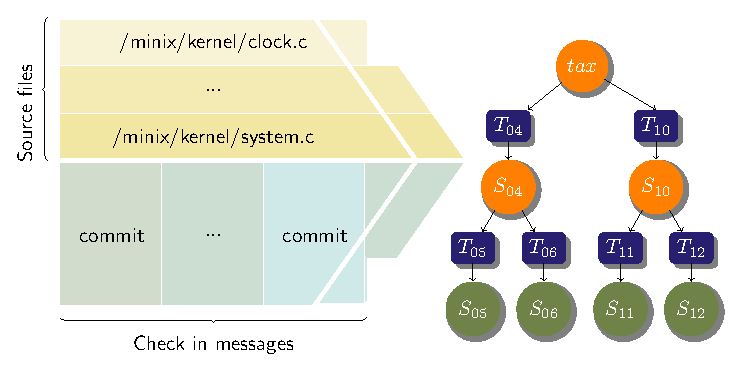
\includegraphics[width=0.9\columnwidth]{figures/framework}
%\caption{Our framework.}
%\label{fig:framework}
%\end{figure}
%
Our system framework consists of 5 steps.
%
%\begin{itemize}
%    \item \textbf{Sentence Clustering}
%
%        We convert each sentence in the reviews into a vector representation 
%        and cluster them in to $N$ clusters of semantically similar sentences.
%
%    \item \textbf{Noise Isolation}
%
%        %As aspects appear as topics in the reviews, 
%        %we use a topic model to infer the potential aspects.
%        To isolate the noises that exist in the sentence cluster,
%	for each sentence cluster we further generate $M$ 
%	topics, resulting in $N\times M$ different word distributions in total.
%
%    \item \textbf{Aspect Inference}
%        
%        We treat each word distribution as a vector and cluster the topics 
%	into $C$ clusters which are the potential aspects. 
%	Here $C$ is purposely set to be larger than $K$. The extra
%	$C-K$ clusters models the redundant aspects.
%        Each cluster contains $N\times M / C$ word distributions, or vectors.
%        We take the mean of these vectors to form $C$ aspect clusters,
%        each being a set of words and their corresponding weights.
%
%    \item \textbf{Cluster Ranking}
%
%        We define a score for the quality of each aspect cluster,
%        and the clusters are ranked by this score.
%
%    \item \textbf{Word Ranking}
%
%        We use WordNet to calculate the semantic distances between the words 
%	in each cluster and adjust the ranking based on the 
%	both the distances and the weights of the words. The top words in each
%	cluster are candidates of the aspect words.
%\end{itemize}
%
%In the following we will explain the motivation and the details of each of
%the five steps. 
%
\subsection{Sentence Clustering}

%One important feature of user reviews is that many topics are 
%compressed into a short paragraph, where each topic corresponds to 
%a potential aspect of the product. 
%A typical hotel review extracted from \figref{fig:tripadvisor} 
%is shown as follows:
%
%\begin{quote}
%Pool is small and only 4 ft but refreshing. Hot tub also there. Staff were super friendly each day. Room was nothing special but clean and comfy. Lots of restaurants and bars nearby. Breakfast was great and despite being a busy weekend there was always a big selection available.
%\end{quote}
%
%In user reviews, topics can shift very quickly.
%Sentences that are close to each other may refer to 
%completely different aspects about the product. Also,
%sentences about the same aspect may not appear in the review consecutively. 
%The existence of such fine-grained semantic shifts in user reviews 
%makes it difficult to apply the the bag-of-word abstraction 
%of normal topic model on reviews.
%Therefore we propose to work on the sentence level instead 
%of the document level, and it would be helpful if we can divide the 
%reviews into topic-oriented segments.
%
%Driven by this observation, in our method the first step is 
%sentence clustering.  For this purpose, 
We represent each sentence in a high-dimensional vector space,
%Instead of using simplistic methods like bag-of-word vector, 
%we leverage a recent development of neural network in natural 
%language processing, the distributed representation.
%In a distributed representation, words and sentences are 
%converted into real-valued vectors.
%The distance of the vectors in the vector space will capture the 
%semantic similarity of the words or sentences.
%In this work we attempt two models, 
using either LSTM (a variant of RNN) or paragraph vector (PV) \cite{le2014distributed}.
%
%\paragraph{Recurrent Neural Network}
%To use RNN for obtaining sentence vectors, 
%we train a neural language model on the review sentences. 
%After the perplexity converges, we use the trained network to 
%process each sentence of the dataset and take the last hidden vector as 
%the vector representation of the sentence. In our method we use a 
%variation of RNN, long-short term memory (LSTM)~\cite{hochreiter1997long} 
%which is reported to have better performance at 
%modeling long sentences \cite{jozefowicz2015empirical}.
%
%\paragraph{Paragraph Vector}
%PV is a simple but powerful extension to Word2vec \cite{mikolov2013distributed} with two components, 
%distributed memory (PV-DM) and distributed bag-of-word (PV-DBOW). 
%The first one is similar to skip-gram in Word2vec and 
%the second is similar to CBOW \cite{mikolov2013distributed}.
%An important advantage of paragraph vector models is that they require 
%no labeled data. Also, it doesn't require human experts to assign weights 
%for words in a paragraph based on linguistic knowledge. 
%The learned vector representations inherit an important property of Word2vec, 
%that is the semantics similarity. Also the final paragraph vector captures the 
%word order information with the part learned from PV-DBOW with the n-gram model.
An advantage of paragraph vector over RNNs is that it can 
leverage trained word vectors, thus requires a smaller training data set. 
%The word vectors can be trained on 
%a much larger corpus so they capture the semantics relationships more 
%accurately.  Consequently, the paragraph vectors can be trained on 
%a relatively small dataset. 
%The performance of paragraph vectors can also be boosted by using pre-trained 
%word vectors that are trained on a larger dataset \cite{mikolov2013linguistic}. 
%%However, previous research show that it is more suitable 
%%to train the word vectors simultaneously for RNNs, 
%%so RNNs cannot leverage the word vectors learned from a larger dataset. 
%Also, the paragraph vector models are simple and 
%don't require the storage of a lot of information. In contrast, for RNN we 
%need to store every state during the forward pass for back-propagation, 
%which is very memory consuming.
%\paragraph{Clustering Sentence Vectors}
We run k-means clustering on the sentence vectors and generate 
$N$ sentence clusters. We then collect the sentences from the same review 
that are clustered together to form smaller fragments of reviews. 
Each original review is divided into several smaller review fragments, 
each belonging to one of the $N$ clusters. As a result, we obtain $N$ 
clusters of review fragments. 

\subsection{Noise Isolation}
There exists noises and overlaps in the clusters formed above.
%The first step, sentence clustering, we might include noise and the sentences 
%within a cluster might not all be about the same aspect. 
%The reason is due to the common occurrences of sentences such as the following
%in the reviews (taken from TripAdvisor):
%
%\begin{quote}
%The room was clean, the staff were friendly, and I would say the price is very reasonable given the proximity to business and leisure destinations around downtown.
%\end{quote}
%
%\begin{quote}
%There is a restaurant just 5 min walk away with nice italian food, pizza was great.
%\end{quote}
%
%In the first sentence multiple aspects are mentioned; in the second sentence, the only aspect is location however lexically it seems to be talking about food.
%With these complicated structures within, 
%it is difficult for RNN or PV to correctly determine the aspects 
%in these sentences. The result is overlaps between clusters about 
%different aspects and noises within each cluster.
%To isolate the noises and resolve such overlap, 
We fix that by applying LDA topic modeling within each sentence cluster, 
treating each review fragment as a document, and generating $M$ smaller topics. 
This will give us in total $N\times M$ topics, or, word distributions. 
%\tabref{table:overlap} shows an example of topics inferred from three
%sentence clusters from hotel reviews and illustrates the overlap problem.
%In this example, five topics were extracted from each sentence cluster, 
%and each row is one topic. It can be seen that the aspects for the 
%three clusters should be {\em room}, {\em location} and {\em price} 
%respectively.
%However, topics shown in boldface font obviously belong to 
%other clusters.  Especially, the last topic of the third cluster 
%appears to be an overlap of more than two clusters.
%The noise isolation step effectively separates the noise topics from other
%topics semantically corehent within a sentence cluster.
%
%\begin{table}[th]
%\centering
%\caption{Topics extracted from three sentence clusters of hotel review.}
%\label{table:overlap}
%\begin{tabular}{|c|l|}
%\hline
%& room bed bedroom size floor \\
%Sentence
%& bedroom room wall size decor \\
%cluster 1
%& room bathroom shower water towel \\
%& room suite size view floor \\
%& room shower area kitchen bed \\\hline
%
%& station minute tube location bus \\
%Sentence
%& location price night place rate\\
%cluster 2
%& location square station street subway\\
%& distance bus subway downtown shopping\\
%& \textbf{restaurant} \textbf{city} \textbf{food} \textbf{buffet} \textbf{place} \\\hline
%
%& price rate service money star\\
%Sentence
%& \textbf{location} \textbf{city} \textbf{star} \textbf{time} \textbf{rate} \\
%cluster 3
%& price service night money city\\
%& price location place night city\\
%& \textbf{location} \textbf{service} \textbf{food} \textbf{price} \textbf{restaurant} \\\hline
%\end{tabular}
%\end{table}


\subsection{Aspect Inference}
\label{sec:topic_clustering}
Each topic is a word distribution, represented by a vector. 
We obtain  more compact representations of those topics by using PCA to 
reduce the topic vectors to 100-dimension.
%We use PCA to reduce the topics vectors to 100-dimension by  
%selecting the 100 words that best distinguish different topics.
Then we perform k-means clustering on the $N\times M$ topics vectors to 
generate $C$ clusters, each containing $(N\times M)/C$ topics.
These are called {\em aspect clusters}.
We set $C$ to be slightly larger than the desired number of product 
aspects $K$, so that the noisy topics can be clustered together and 
later discarded. 
%In an experiment we will evaluate the influence of this redundant clusters on 
%the quality of the final aspects.
%
%\begin{table}[th]
%\caption{Aspect clusters extracted from hotel reviews.
%Each row shows the candidate words of an aspect, sorted by the weight of each word.}
%\label{table:step3}
%\centering
%\begin{tabular}{|l|} \hline
%breakfast, meal, food, tasty, dinner, morning, coffee, tea \\\hline
%room, night, time, bed, day, bathroom, staff, area, place \\\hline
%staff, desk, service, friendly, reception, concierge, helpful \\\hline
%close, city, location, place, central, station, bus, street\\\hline
%bed, shower, spacious, room, size, bathroom, bedroom, floor \\\hline
%price, room, check, night, money, city, location, star, service \\\hline
%location, price, room, night, place, rate, money, time, city  \\\hline
%\end{tabular}
%\end{table}
%
%Finally, for each cluster we take the mean of the $(N\times M)/C$ 
%topics and normalize it
%for the word distribution of that cluster.
%Some example aspect clusters extracted from hotel reviews are 
%shown in \tabref{table:step3}.

\subsection{Cluster Ranking}

We rank the clusters by how ``distinct'' each cluster is from other clusters. 
If a cluster is similar to other clusters, it is considered redundant and of
low quality. We discard $C-K$ least distinct clusters.


%For the $i$th cluster $C_i$ ($i\in [1, C]$), 
%the distinctiveness score $S(i)$ is defined by:
%
%\begin{align}
%S(i) &= \sum_{w\in C_i} S_i(w) \nonumber\\ 
%     &= \sum_{w\in C_i} \log\left(\frac{f_i(w)}{\sum_{j\neq i} f_j(w)}\right)\nonumber \\
%     &= \sum_{w\in C_i}\left[\log f_i(w) - \log\sum_{j\neq c} f_j(a)\right]
%\end{align}
%
%\begin{table}[t]
%\caption{Aspect clusters ranked by distinctiveness score.
%Potential aspect words are boldfaced.}
%\label{table:clustersranked}
%\centering
%\begin{tabular}{|l|} \hline
%\textbf{staff}, desk, \textbf{service}, friendly, reception, concierge, helpful \\\hline
%breakfast, meal, \textbf{food}, tasty, dinner, morning, coffee, tea \\\hline
%\textbf{price}, room, check, night, money, city, location, star, service \\\hline
%bed, shower, spacious, \textbf{room}, size, bathroom, bedroom, floor \\\hline
%close, city, \textbf{location}, place, central, station, bus, street \\\hline
%\textcolor{red}{room, night, time, bed, day, bathroom, staff, area, place} \\\hline
%\textcolor{red}{location, price, room, night, place, rate, money, time, city} \\\hline
%\end{tabular}
%\end{table}
%
\subsection{Word Ranking}
\label{sec:word_ranking}

We rank the words in each cluster 
by considering two factors (similar to TF-IDF): 
the representativeness of the word to the host
cluster; the number of times the word appears in other clusters. 
The most representative word in each cluster
is assumed to be the closest to the centroid of the word cluster.
The distance between two words is the inverse of 
cosine similarity between the word2vec
vectors of the two words.
Then we process the clusters in the order of 
the cluster ranking given in the last step.
When we calculate the score for word $x$ cluster $C_i$,
we also consider the scores of word $x$ in clusters $C_1$ to $C_{i-1}$, 
where the scores have already been calculated. 
We prevent the duplicate aspect words by subtracting the scores 
of $C_1$ to $C_{i-1}$, from the score of $C_i$.
%The score of word $x$ in the $i$th cluster $C_i$ is thus defined by:
%
%\begin{equation}
%s_i(x) = u_i(x) \sum_{y\in C_i}\hat{x}\cdot \hat{y} - \sum_{j=1}^{i-1}s_j(x),
%\label{eq:wordscore}
%\end{equation}
%where $\hat{x}$ is the vector representation of x; $u_i(x)$ is the weight of $x$ in cluster $C_i$.
The words in each cluster is thus ranked by this final score.

\section{Evaluation}
\label{sec:experiments}

We evaluated our framework
against a number of baselines including the state-of-the-art approaches.
%in the end-to-end aspect extraction task.
Our dataset is reviews for 15 categories of product or service crawled from
e-commerce sites such as Amazon.com and Yelp. 
%The review content is plain English text and we do not use any labels 
%for training our model. We use human labels for evaluation. 
%The product categories, their sources and the sizes of the review datasets
%are summarized in \tabref{table:dataset}
%
%\begin{table}[th]
%\centering
%\caption{Dataset summary.} 
%\label{table:dataset}
%\begin{tabular}{|c|c|r|r|}
%\hline
%Product type & Source & No. of Reviews & No. of Words \\ \hline \hline
%hotel        & TripAdvisor & 27145   & 210 \\\hline
%mobile phone & Amazon & 3716    & 136 \\\hline
%mp3 player   & Amazon & 2745    & 128 \\\hline
%laptop       & Amazon & 5471    & 97  \\\hline
%tv           & Amazon & 1237    & 102 \\\hline
%shoes        & Amazon &1748    & 82  \\\hline
%headphone    & Amazon & 1647    & 122 \\\hline
%gps          & Amazon & 1726    & 72  \\\hline
%transportation & Yelp & 3077  & 131 \\\hline
%restaurant   & Yelp & 4016    & 176 \\\hline
%gym          & Yelp & 2481    & 230 \\\hline
%shopping     & Yelp & 2718    & 123 \\\hline
%car dealer   & Yelp & 2839    & 190 \\\hline 
%movie        & Pang et al. \cite{pang2002thumbs} & 3000    & 194 \\\hline
%car          & Cars.com & 1074    & 147 \\\hline
%\end{tabular}
%\end{table}
%
%
%For evaluation, we ask 5 college students proficient with English 
%to annotate ground truth
%aspect words for each product category. For each category, 
%we ask them to provide 5 different words that cover the most important 
%aspects of the corresponding product or service. The labels provided by the
%5 annotators are aggregated together without removing duplicated words, 
%so we have 25 words in total. 
%When evaluating the models, 
%we compare the 5 aspect words generated by the models with those provided 
%by the annotators. 
%We calculate the portion of words among the 25 labels that 
%are correctly generated by the model as the accuracy of the model.
%The ground-truth labels for two product categories are shown 
%in \tabref{table:labels}.
%
%
%\begin{table}[th]
%\centering
%\caption{Labels for hotel and shopping. Each row is provided by one annotator.}
%\label{table:labels}
%\begin{tabular}{|c|l|}
%\hline
%\multirow{5}{*}{hotel}
%& room price location service utility \\
%& room service price food location  \\
%& sleep service room price location  \\
%& location price bedroom bath staff  \\
%& room price bath staff location  \\\hline
%
%\multirow{5}{*}{shopping}
%& location product service price environment \\
%& product price service location ambience \\
%& price food location size facility \\
%& sales location food service environment \\
%& price location service facility food \\\hline
%\end{tabular}
%\end{table}
%
%\subsubsection{Parameter Tuning}
We conduct a few experiments to determine the following
parameter settings: $N=10$, $M=10$, $C=K+2$, i.e. at most two extra clusters.

We compare 5 models in our experiments, 
LDA as a simple baseline, 
D-PLDA \cite{moghaddam2012design} as a representative for joint 
aspect-sentiment models, MG-LDA \cite{titov2008modeling} as 
a representative for aspect extraction topic model,
and two variations of our model LSTM and PV. 
We run the 5 models on the review data of each product type separately. 
For the main experiment, the number of aspects is fixed to 5.

%\begin{figure*}[th]
%\centering
%\includegraphics[width=1.9\columnwidth]{figures/results}
%\caption{Accuracies from different models.}
%\label{fig:results}
%\end{figure*}
%In the end-to-end evaluation, we compare the performance of our models on aspect extraction with three other models as mentioned above. The results are shown in \figref{fig:results}. 
By the accuracy, our two models out-performed all other models in 13 out of 15 
categories. The PV model performs better LSTM, 
which is consistent to our earlier analysis. \tabref{table:hotel_aspect_words}
shows the 5 aspect words by each model for hotel reviews.

\begin{table}[th]
\centering
\small
\caption{Top aspect words for hotels by different models}
\label{table:hotel_aspect_words}
\begin{tabular}{|l|l|} \hline
Ours(PV) & staff, food, price, room, location \\ \hline
Ours(LSTM) & service, location, time, food, bed\\ \hline
MG-LDA & shower, time, food, room, price\\ \hline
DP-LDA & service, station, check, coffee, bed \\ \hline
LDA & stay, location, room, staff, room \\ \hline
\end{tabular}
\end{table}
 
\section{Demo Scenarios}
We present a web demo which depicts the following scenario.
The user logs on and selects
a product type, e.g. ``cell phones'', from a predefined set of categories,  
and sets the number of aspects $K$. 
Then the user clicks the ``generate" button to extract $K$ aspect words for the selected product type.
Upon this, the system computes the review summaries of all cell phones. 
%Upon this, the system shows the $K$ precomputed aspect words for that
%product type, computed from the many user reviews about ``cell phones''. 
%Then the user clicks a button to ``generate review summaries'', which presents
%the review summaries of all cell phones in
%the system. 
Each summary contains the aspects and their scores, computed from the sum of
sentiment scores (1, 0 or -1) against each aspect using LSTM trained on
Stanford Sentiment Treebank~\cite{socher2013recursive}. 
The user may filter out some of the 
results by using the search box (see \figref{fig:summary1}). 
If the user wishes to understand why a product receives a score for a 
certain aspect, they can click on the ``xxx customer reviews'' link
and be directed to the original review snippets with the aspect words and 
sentiment words highlighted. The review snippets by can further grouped by
aspects by clicking on the tabs (see \figref{fig:summary2}). 

\begin{figure}[th]
\includegraphics[width=\columnwidth]{figures/demo1.png}
\caption{Automatically generated 6 aspects for cell phones}
\label{fig:summary1}
\end{figure}

\begin{figure}[th]
\includegraphics[width=\columnwidth]{figures/demo21.png}
\caption{Review snippets displayed by the aspects}
\label{fig:summary2}
\end{figure}


%The second and a minor scenario enables the user to examine the dynamic change
%in aspect words over time for each product type. The system shows a time line,
%annotated with different sets of aspect words, by configurable time periods,
%e.g., every month, 6 months or a year.  
 
\bibliographystyle{IEEEtran}
\bibliography{master}
\end{document}

%\section{Related Work}
This section surveys previous works on question generation and tree encoding
respectively.

Text question generation has attracted the attention 
after the work of ~\citeauthor{du2017learning}~\shortcite{du2017learning}, who uses deep seq2seq model 
to generate questions from a raw text paragraph. 
Before that, text question generation relied heavily on hand-craft 
question patterns~\cite{HeilmanS10,LabutovBV15,MostowC09} which is time and 
labor consuming. 

However, this pure seq2seq model is not focused and 
has no control over part in the paragraph to generate question. 
~\citeauthor{zhou2017neural}~\shortcite{zhou2017neural} proposed to encode 
key phrase information using binary indicators to generate 
key-aware questions and they assumes the answer to be key phrase. 
Considering key phrase (answer) is unavailable in reality, 
~\citeauthor{SubramanianWYT17}~\shortcite{SubramanianWYT17} applied 
a two-stage approach. First, key phrases are extracted by 
pointer network~\cite{ptrnet}. Second, 
key phrases are encoded in the same way as 
Zhou et al. With the intuition that questions could be asked in many ways, 
~\citeauthor{Yao2018vae}~\shortcite{Yao2018vae} used conditional-VAE to 
increase the diversity of questions. More recently, models with 
auxiliary feature information~\cite{HarrisonW18} helped improve 
the question quality. Structure question generation aims at 
converting structured data such as triples in knowledge graph to questions. 
~\citeauthor{SerbanGGACCB16}~\shortcite{SerbanGGACCB16} proposed a model to generate factoid questions from knowledge base triples.  None of the above work
considered using parse tree structures to aid question generation process,
which is the focus of this paper.

Sequential RNN model takes sentence as a sequence of words, 
ignoring the syntactic information. In order to utilize
such syntactic information with sequential information, 
~\citeauthor{tai2015improved}~\shortcite{tai2015improved} proposed Tree-LSTM to 
encode the binary parse tree recursively in a bottom-up fashion to 
classify sentiment. In text generation task, 
\citeauthor{eriguchi2016tree}~\shortcite{eriguchi2016tree} 
proposed a tree-to-sequence model with attention mechanism to do 
machine translation and 
~\citeauthor{liang2018automatic}~\shortcite{liang2018automatic} proposed a 
tree-to-sequence model which could handle arbitrary trees, 
to do code comment generation. Our work is inspired by these previous
attempts and we are first to adapt structure encoded neural models to
textual question generations.
%\section{Conclusion}
\label{sec:conclude}
In this work,
we propose a new data creation method to generate
 a semi-structured synthetic training data for 
opinion summarization,
which is known for lacking training data.
\cut{We showed that by extracting an aspect-opinion pairs and 
implicit sentences from multiple reviews
first and then synthesizing them into semi-structured data, we achieve
better performance on opinion summarization.}
%\KZ{It is critical to show in your experiments that the proposed
%synthetic data is better than other possible alternatives.}, 
We also designed an aspect-guided model with opinion-aspect pair encoder and implicit sentence encoder.
The results showed that
the proposed model can make full use of semi-structured data
and generate high-quality summaries.





\bibliographystyle{abbrv}
\bibliography{../bibs/wiki,../bibs/image}
%\bibliography{../bibs/image}

\end{document}
